%\documentclass{article}
%\documentclass[hyperref={colorlinks=true}]{beamer}
\documentclass[handout,hyperref={colorlinks=true}]{beamer}


%%%%%%%%%%%%%%%%%%%%%%%%%%%%%%Paquetes%%%%%%%%%%%%%%%%%%%%%%%%%%%%%%%%%%%%%%%%%%%%%%%5
%%%%%%%%%%%%%%%%%%%%%%%%%%%%%%%%%%%%%%%%%%%%%%%%%%%%%%%%%%%%%%%%%%%%%%%%%%%%%%%%%%%%%

\usepackage{pgfpages}
%\pgfpagesuselayout{2 on 1}[a4paper,border shrink=5mm]
\usepackage{empheq}
\usepackage[spanish]{babel}
\usepackage[utf8x]{inputenc}
\usepackage{times}
\usepackage[T1]{fontenc}
\usepackage{amssymb,amsmath}
\usepackage{enumerate}
\usepackage{verbatim}
\usepackage{ esint }
%\usepackage{pst-all}
%\usepackage{pstricks-add}
\usepackage{array}
%\usepackage[T1]{fontenc}
\usepackage{animate}
%\usepackage{media9}
\usepackage{xparse}
\usepackage{listings}
\usepackage{ wasysym }
\usepackage{sagetex}
\usepackage{hyperref}




%%%%%%%%%%%%%%%%%%%%%%%%%Configuracion listing
\lstdefinelanguage{Sage}[]{Python}
{morekeywords={False,sage,True},sensitive=true}
\lstset{
  frame=none,
  showtabs=False,
  showspaces=False,
  showstringspaces=False,
  commentstyle={\ttfamily\color{dgreencolor}},
  keywordstyle={\ttfamily\color{dbluecolor}\bfseries},
  stringstyle={\ttfamily\color{dgraycolor}\bfseries},
  language=Sage,
  basicstyle={\fontsize{8pt}{8pt}\ttfamily},
  aboveskip=.3em,
  belowskip=0.1em,
  numbers=none,
  numberstyle=\footnotesize
}


 


%%%%%%%%%%%%%%%%%%%%%%%%Colores
\definecolor{myblue}{rgb}{.8, .8, 1}
\definecolor{dblackcolor}{rgb}{0.0,0.0,0.0}
\definecolor{dbluecolor}{rgb}{0.01,0.02,0.7}
\definecolor{dgreencolor}{rgb}{0.2,0.4,0.0}
\definecolor{dgraycolor}{rgb}{0.30,0.3,0.30}
\newcommand{\dblue}{\color{dbluecolor}\bf}
\newcommand{\dred}{\color{dredcolor}\bf}
\newcommand{\dblack}{\color{dblackcolor}\bf}










%%%%%%%%%%%%%%%%%%%%%%%%%%Nuevos comandos entornos%%%%%%%%%%%%%%%%%%%%%%%%%%%%%%%%
%%%%%%%%%%%%%%%%%%%%%%%%%%%%%%%%%%%%%%%%%%%%%%%%%%%%%%%%%%%%%%%%%%%%%%%%
\newenvironment{demo}{\noindent\emph{Dem.}}{$\square$ \newline\vspace{5pt}}
\newcommand{\com}{\mathbb{C}}
\newcommand{\dis}{\mathbb{D}}
\newcommand{\rr}{\mathbb{R}}
\newcommand{\oo}{\mathcal{O}}
\renewcommand{\emph}[1]{\textcolor[rgb]{1,0,0}{#1}}
\newcommand{\der}[2]{\frac{\partial #1}{\partial #2}}
\renewcommand{\v}[1]{\overrightarrow{#1}}
\renewcommand{\epsilon}{\varepsilon}
\newlength\mytemplen
\newsavebox\mytempbox
\makeatletter
\newcommand\mybluebox{%
    \@ifnextchar[%]
       {\@mybluebox}%
       {\@mybluebox[0pt]}}

\def\@mybluebox[#1]{%
    \@ifnextchar[%]
       {\@@mybluebox[#1]}%
       {\@@mybluebox[#1][0pt]}}

\def\@@mybluebox[#1][#2]#3{
    \sbox\mytempbox{#3}%
    \mytemplen\ht\mytempbox
    \advance\mytemplen #1\relax
    \ht\mytempbox\mytemplen
    \mytemplen\dp\mytempbox
    \advance\mytemplen #2\relax
    \dp\mytempbox\mytemplen
    \colorbox{myblue}{\hspace{1em}\usebox{\mytempbox}\hspace{1em}}}

\makeatother
\DeclareDocumentCommand\boxedeq{ m g }{%
    {\begin{empheq}[box={\mybluebox[2pt][2pt]}]{equation}% #1%
        \IfNoValueF {#2} {\label{#2}}%
       #1
       \end{empheq}
    }%
}
\DeclareMathOperator{\atan2}{atan2}
\DeclareMathOperator{\sen}{sen}
\newtheorem{teorema}{Teorema}[section]
\newtheorem{lema}[teorema]{Lema}
\newtheorem{corolario}[teorema]{Corolario}
\newtheorem{proposicion}[teorema]{Proposici\'on}
\newtheorem{definicion}[teorema]{Definici\'on}
%%%%%%%%%%%%%%%%%%%%%%%%%%%%%%%%%%%%%%%%%%%%%%%%%%%%%%%%%%%%%%%%%%%%%%%%%%%%%%%%%%%%%%%%%%%%%%%%%%%%%%%%%%%




%%%%%%%%%%Para escibir en clase articulo o similar
% \usepackage{color}
% \newcommand{\nl}{ }
% \renewenvironment{frame}[1]{}{}
% \newcommand{\qed}{$\square$}
% %\newcommand{\defverbatim}{\def{#1}}
% \newenvironment{block}[1]{\textbf{#1}}{}
% \title{Ecuaciones lineales de segundo orden}
% \author{Fernando Mazzone}
% 




%%%%%%%%%%%%%%%%%%%%%%%Para clase beamer
\newcommand{\nl}{\onslide<+-> }
% \mode<all>
% {
%   \usetheme{Boadilla}
%   % oder ...
%  
%   \setbeamercovered{wolverine}
%   % oder auch nicht
% }


\mode<handout>{
  \usetheme{default}
  %\setbeamercolor{background canvas}{bg=black!5}
  \pgfpagesuselayout{4 on 1}[letterpaper,landscape,border shrink=2.5mm]
}

% \mode<all>{
%   \usetheme{default}
%   %\setbeamercolor{background canvas}{bg=black!5}
%   \pgfpagesuselayout{4 on 1}[letterpaper,landscape,border shrink=2.5mm]
% }

\title[Ecuaciones lineales de segundo orden] % (optional, nur bei langen Titeln nötig)
{%
 Ecuaciones lineales de segundo orden
}



\author[] % (optional, nur bei vielen Autoren)
{Fernando Mazzone}

\institute[Depto de Matemática] % (optional, aber oft nötig)
{
 Depto de Matemática\\
Facultad de Ciencias Exactas Físico-Químicas y Naturales\\
Universidad Nacional de Río Cuarto}


\subject{Ecuaciones Diferenciales}

%%%%%%%%%%%%%%%%%%%%%%%%%%%%%%%%%%%%%%%%%%%%%%%%%%%%%%%%%%%%%%%%%%%%%%%%%%%%%%%%%%%%%%




\begin{document}

\begin{frame}
  \maketitle
  \begin{center}
   
\includegraphics[scale=0.2]{imagenes/unrc.jpg}
   \end{center}
\end{frame}










\begin{frame}{Introducción}
\begin{block}{Ecuación lineal general de segundo orden}
\boxedeq{\frac{d^2y}{dx^2}+p(x)\frac{dy}{dx}+q(x)y=r(x),}{ec_2_gen}
donde $p,q,r$ son funciones definidas en un intervalo $I=(a,b)$ de $\rr$ con valores en $\rr$. 
\end{block}
Si $r\equiv 0$ se llama homogénea
\boxedeq{\frac{d^2y}{dx^2}+p(x)\frac{dy}{dx}+q(x)y=0,}{ec_2_gen_hom}
\end{frame}


\begin{frame}{Introducción}
\nl \begin{block}{Teorema de existencia y unicidad de soluciones}
 Supongamos $p,q,r$ continuas sobre $I$. Sean $x_0\in I$ e $y_0,y_1\in\rr$ dados. Entonces existe una única solución del PVI
 \[\left\{
 \begin{array}{l l l}
   \frac{d^2y}{dx^2}+&p(x)\frac{dy}{dx}+q(x)y=r(x),&x\in I\\
   y(x_0)&=y_0&\\
   y'(x_0)&=y^1_0&\\ 
  \end{array}\right.
\]


\end{block}
\nl \textbf{Demostración.} Más adelante.
\end{frame}


\section{Estructura del conjunto de soluciones}

\begin{frame}{Ecuaciones homogéneas}
\nl\begin{block}{Teorema}
 Si $y_1$ e $y_2$ son soluciones de \eqref{ec_2_gen_hom} y $c_1,c_2\in\rr$ entonces $c_1y_1+c_2y_2$ es solución. Vale decir, el conjunto de soluciones 
 es un espacio vectorial. En particular $y\equiv 0$ es una solución, a la que llameremos \emph{trivial}.

 

\end{block}

\nl\textbf{Demostración} 
 El operador 
 \[L[y]:=y''+py'+qy\]
es lineal, por consiguiente
$L[c_1y_1+c_2y_2]=c_1L[y_1]+c_2L[y_2]=0.$\qed
\end{frame}



\begin{frame}{Ecuaciones no homogéneas}
\nl\begin{block}{Teorema}
 Supongamos que $y_p$ es una solución particular de \eqref{ec_2_gen} y que $y_g=y_g(x,c_1,c_2)$ es una solución
 general de \eqref{ec_2_gen_hom}. Entonces $y=y_p+y_g$ es solución general de \eqref{ec_2_gen}.
\end{block}

\nl\textbf{Demostración} 
 El operador 
 \[L[y]:=y''+py'+qy\]
es lineal, por consiguiente
$L[y_g+y_p]=L[y_g]+L[y_p]=0+r=r.$
Recíprocamente supongamos $y$ solución de $L[y]=r$, entonces
$L[y-y_p]=L[y]-L[y_p]=r-r=0.$
Luego debe haber $c_1$ y $c_2$ con $y(x)-y_p(x)=y_g(x,c_1,c_2)$.\qed 
 
\end{frame}


\begin{frame}{Ecuaciones homogéneas}
\nl Volviendo a las ecuaciones homogéneas, supongamos que tenemos dos soluciones de \eqref{ec_2_gen_hom} $y_1$ e $y_2$. Entonces la expresión 
\begin{equation}\label{comb_lin}
   c_1y_1+c_2y_2,\quad c_1,c_2\in\rr
\end{equation}
es solución también. \nl Notar que en la expresión aparecen dos constantes y habíamos dicho que era de esperar que la solución general de una ecuación de orden 2 contuviese
precisamente dos constantes de integración. De modo que podemos conjeturar que \eqref{comb_lin} es solución general de \eqref{ec_2_gen_hom}. 

\nl Hay una situación especial, si, por ejemplo, $y_1=ky_2$, $k\in\rr$,entonces $c_1y_1+c_2y_2=(c_1k+c_2)y_2=cy_2$. Vale decir la combinación lineal \eqref{comb_lin}
termina siendo sólo combinación lineal de la función $y_2$ y por ende siendo esencialmente una expresión uniparamétrica.  
\end{frame}

\begin{frame}{Independencia lineal}
 
\begin{block}{Definición de independencia lineal}
 Un conjunto finito de funciones $\{y_1,\ldots,y_n\}$ se dirá linealmente independiente sobre un conjunto $I$, 
 si la única solución de $c_1y_1(t)+\cdots+c_ny_n(t)=0$, para $t\in I$, es $c_1=c_2=\cdots=c_n=0$.
\end{block}

\end{frame}

\begin{frame}{Independencia lineal}
 
\begin{block}{Definición wronskiano}

Dadas $n$ fuciones  $\{y_1,\ldots,y_n\}$ con dominio $I$ el wronskiano $W(x)=W(y_1,y_2,\ldots,y_n)(x)$ de estas funciones en un punto $x\in I$ se define por
\boxedeq{W(x)=\det\begin{pmatrix}
                                  y_1(x) & y_2(x) & \cdots &y_n(x)\\
                                  y_1'(x) & y_2'(x) & \cdots &y_n'(x)\\
                                  \vdots & \vdots &\ddots& \vdots\\
                                  y_1^{(n-1)}(x) & y_2^{(n-1)}(x) & \cdots &y_n^{(n-1)}(x)\\
                               \end{pmatrix}}{wronskiano}
\end{block}
\end{frame}


\begin{frame}{Independencia lineal}
\nl\begin{block}{Lema. Propiedades Wronskiano I}
Sea $\{y_1,\ldots,y_n\}$ un conjunto de $n$ funciones. Si existe un $x_0\in I$ con $W(x_0)\neq 0$ entonces   $\{y_1,\ldots,y_n\}$ son
linealmente independientes
\end{block}

\nl\textbf{Demostración.} Supongamos que $c_1y_1+\cdots+c_ny_n\equiv 0$. Derivando $n-1$ veces esta igualdad y evaluando el resultado en $x_0$ obtenemos
\[
 \begin{split}
    c_1y_1(x_0)+\cdots+c_ny_n(x_0)&=0\\
    c_1y_1'(x_0)+\cdots+c_ny'_n(x_0)&=0\\
    \vdots \quad& \quad\vdots\\
    c_1y_1^{(n-1)}(x_0)+\cdots+c_ny^{(n-1)}_n(x_0)&=0\\
 \end{split}
\]


\end{frame}

\begin{frame}{Independencia lineal}
 Las igualdades anteriores dicen que el vector $(c_1,\ldots,c_n)^t$ pertenece al nucleo de la matriz 
\[
\begin{pmatrix}
                                  y_1(x_0) & y_2(x_0) & \cdots &y_n(x_0)\\
                                  y_1'(x_0) & y_2'(x_0) & \cdots &y_n'(x_0)\\
                                  \vdots & \vdots &\ddots& \vdots\\
                                  y_1^{(n-1)}(x_0) & y_2^{(n-1)}(x_0) & \cdots &y_n^{(n-1)}(x_0)\\
                               \end{pmatrix}
\]
Como por hipótesis la matríz es no singular, debe ocurrir que $c_1=c_2=\cdots c_n=0$. \qed

\end{frame}
\begin{frame}{Fórmula de Abel}
\begin{block}{Teorema. Propiedades wronskiano II}
Supongamos que  $y_1$ e $y_2$  son solución de 
\begin{equation}\label{eq2orden}\frac{d^2y}{dx^2}+p(x)\frac{dy}{dx}+q(x)y=0,\quad x\in I=(a,b)\end{equation}
 Entonces existe $c\in\rr$ que satisface
\boxedeq{W(y_1,y_2)(x)=ce^{-\int p dx}.}{formu_abel}
Esta expresión  se denomina \href{http://en.wikipedia.org/wiki/Abel's_identity}{fórmula de Abel}. En particular vale que
\[\exists x_0\in I: W(x_0)\neq 0 \Longleftrightarrow \forall x\in I: W(x)\neq 0 .\]
\end{block}
\end{frame}


\begin{frame}{Demostración fórmula Abel}
\textbf{Demostración.} Tenemos que 
\[W(x)=y_1(x)y_2'(x)-y_1'(x)y_2(x).\]
Derivando y usando \eqref{eq2orden}
\[\begin{split}W'(x)&=y_1y_2''-y_1y_2''\\
   &=y_1(-py_2'-qy_2)-y_2(-py_1'-qy_1)\\
   &=-pW.
  \end{split}
\]
Vale decir $W$ resuelve la ecuación $W'=-pW$ la cual es facilmente resoluble, mostrando su resolución que se satisface \eqref{formu_abel}\qed 


\end{frame}
 
 
\begin{frame}{Independencia y wronskiano}
\nl\begin{block}{Propiedades wronskiano III}
 Sean $y_1$ e $y_2$ soluciones de \eqref{eq2orden}. Entonces son equivalentes
 \begin{enumerate}
  \item\label{item1} $y_1$ e $y_2$ son linealmente indepenientes en $I$. 
  \item\label{item2} $W(y_1,y_2)(x)\neq 0$ para todo $x\in I$.
 \end{enumerate}
\end{block}
\nl\textbf{Demostración.}  Que \ref{item2} implica \ref{item1} es consecuencia de la propiedad del wronskiano I. 
Veamos que \ref{item1} implica \ref{item2}. Supongamos que exista un $x_0$ con $W(x_0)=0$. Esto quiere decir  que una de las columnas
de la matríz wronskiana en $x_0$ es múltiplo de la otra. Supongamos que $y_2(x_0)=ky_1(x_0)$ e $y'_2(x_0)=ky'_1(x_0)$. Esto quiere decir que $y_2$ y $ky_1$
resuelven el mismo pvi. Por lo tanto $y_2(x)=ky_1(x)$ para todo $x$. Lo que nos dice lo contrario de \ref{item1}\qed

\end{frame} 
 
\begin{frame}{Estructura soluciones ecuaciones homogéneas}
\begin{block}{Teorema, estructura del conjunto de soluciones ecuación lineal de segundo orden homogénea}
Si $y_1$ e $y_2$ son soluciones linealmente independientes de 
\[\frac{d^2y}{dx^2}+p(x)\frac{dy}{dx}+q(x)y=0,\quad x\in I=(a,b)\]
entonces
\boxedeq{ y(x,c_1,c_2)=c_1y_1+c_2y_2}{comb_lin2}
es solución general.
\end{block}

\end{frame}

\begin{frame}{Estructura soluciones ecuaciones homogéneas}
\textbf{Demostración.} Que la expresión \eqref{comb_lin2} es solución ya lo hemos dicho.   Restaría ver que cualquier solución se escribe como en \eqref{comb_lin2}. 
Sea $y$ cualquier solución y $x_0\in I$. La matriz wronskiana
\[\begin{pmatrix}
   y_1(x_0)  & y_2(x_0)\\
   y'_1(x_0)  & y'_2(x_0)\\   
  \end{pmatrix}
\]
Es no singular dado que el determinante es no nulo. Por este motivo el sistema
\[ \begin{split}
  c_1 y_1(x_0) + c_2y_2(x_0) &=y(x_0)\\
   c_1y'_1(x_0)  + c_2y'_2(x_0) &=y'(x_0)\\
  \end{split}
\]
tiene solución para $c_1$ y $c_2$. 
\end{frame}


\begin{frame}{Estructura soluciones ecuaciones homogéneas}
De este modo vemos que la función  $c_1y_1+c_2y_2$ resuelve el PVI

 \[\left\{
 \begin{array}{l l l}
   \frac{d^2z}{dx^2}+&p(x)\frac{dz}{dx}+q(x)z=0,&x\in I\\
   z(x_0)&=y(x_0)&\\
   z'(x_0)&=y'(x_0)&\\ 
  \end{array}.\right.
\]
Evidentemente $y$ es solución también, por el Teorema de Existencia y Unicidad vemos que $y=c_1y_1+c_2y_2$ \qed
\end{frame}

\section{Reducción de orden}
\begin{frame}{Reduccción de orden}
\nl Como conclusión de los anterior, vemos que si queremos resolver \eqref{eq2orden} debemos conseguir  dos soluciones linealmente independientes.

\nl Suponiendo que ya contamos con una solución no trivial vamos a describir un método 
  que posibilita  encontrar otra solución $y_2$ linealmente independiente de $y_1$. 
  
\nl El método consiste en proponer que $y_2$ se escribe

\[\boxed{y_2(x)=v(x)y_1(x)}.\]


\end{frame}


\begin{frame}{Reduccción de orden}
Luego
\[
 \begin{split}
    0&=y_2''+py_2'+qy_2\\
    &=y_1v''+2v'y_1'+vy_1''+pv'y_1+pvy_1'+qvy_1\\
    &=y_1 v''+(2y_1'+py_1)v'+v(y_1''+py_1'+qy_1)\\
    &=y_1 v''+(2y_1'+py_1)v'
 \end{split}
\]
La fórmula anterior es nuevamente una ecuación de segundo orden para $v$, 
pero en este caso afortunadamente contamos con herramientas para resolverla puesto que se trata de una ecuación donde la 
variable dependiente $v$ no aparece explícitamente, sino que aparecen sus derivadas $v'$ y $v''$. Hay que intentar la sustitución $w=v'$


\end{frame}
 
 
\begin{frame}{Reduccción de orden}
Luego
\[
 y_1w''+(2y_1'+py_1)w=0
\]
Recordar que $y_1$ la asumimos conocida y que $p$ es obviamente conocida, así $2y_1'+py_1$ es una funcióon conocida. La ecuación es una ecuación lineal homogénea de primer orden. 
Usando la fórmula para resolver este tipo de ecuación dada en nuestra 
\href{https://github.com/fdmazzone/Material-Ecuaciones-Diferenciales/blob/master/uni2.pdf?raw=true}{presentación anterior}, obtenemos
\[w(x)=Ce^{-\int \frac{y_1'}{y_1}+p dx}=Ce^{-2\ln|y_1|}e^{-\int p dx}=C\frac{1}{y_1^2}e^{-\int p dx} \]
Es suficiente encontrar sólo una función $v$, de allí podemos tomar $C=1$. 
\boxedeq{w(x)= \frac{1}{y_1^2}e^{-\int p dx}\Longrightarrow v(x)= \int \frac{1}{y_1^2}e^{-\int p dx}dx }{reduc_orden}



\end{frame} 

\begin{frame}{Reduccción de orden}
\nl Otra manera de testear la independencia lineal de dos funciones $y_1$ e $y_2$ es notar que si fueran linealmente dependientes e $y_1\neq 0$ 
en un conjunto $J\subset I$ entonces $y_2/y_1$
sería constante.  
\nl Luego uno chequearía independencia si comprobase que $y_2/y_1$ no es constante en algún subdominio $J\subset I$. 

\nl En el caso anterior $y_2/y_1=v$, luego 
deberíamos tener $v$ no constante sobre algún subconjunto $J$. Pero $v$ constante implicaría $y_1^{-2}e^{-\int pdx}=0$ y esto claramente no ocurre. De modo que por el
método anterior encontramos dos soluciones independientes.   





\end{frame} 


 \section{Ecuaciones homogéneas con coeficientes constantes}
\begin{frame}{Ecuaciones homogéneas con coeficientes constantes}
 
 Consideramos la ecuación
 
 \boxedeq{y''+py'+qy=0,\quad p,q\in\rr}\label{2orden_coef_ctes}
    
 Propongamos una solución de la forma 
 \[\boxed{y(x)=e^{\lambda x},\quad \lambda\in\mathbb{C}}\]
 Reemplazando en la ecuación
 \[(\lambda^2+\lambda p+q)e^{\lambda x}=0.\]
Se debe satisfacer la llamada \emph{ecuación característica}
\boxedeq{\lambda^2+p\lambda+q=0}{ecua_carac} 
\end{frame}

\begin{frame}{Ecuaciones homogéneas con coeficientes constantes}
Tenemos tres casos acorde al valor de $\Delta:=p^2-4c$

\nl 1)\textbf{$\boxed{\Delta=p^2-4c>0}$, raices reales distintas $\lambda_1$, $\lambda_2$}. Este es el caso más sencillo de todos, obtenemos las soluciones
\[y_1(x)=e^{\lambda_1 x}\quad\text{y}\quad y_2(x)=e^{\lambda_2 x}.\]
Para chequear la independencia
\[\frac{y_2}{y_1}=e^{(\lambda_2-\lambda_1)x}\neq\text{cte}.\]
Luego 
\boxedeq{y(x,c_2,c_2)=c_1e^{\lambda_1 x}+c_2e^{\lambda_2 x}.}{sol_gen1}
es solución general
\end{frame}

\begin{frame}{Ecuaciones homogéneas con coeficientes constantes}
2) \textbf{$\boxed{\Delta=p^2-4c<0}$, raices complejas conjugadas $\lambda_1=\mu+i\nu$, $\lambda_2=\mu-i\nu$, $\mu,\nu\in\rr$}.

Proponemos una solución de la forma
\[
 y(x)=e^{\mu x}v(x)
\]

Hagamos los cálculos con SAGE
 



\end{frame}

\defverbatim[colored]\lstI{ 
\begin{lstlisting}
sage: x,p,q=var('x,p,q')
sage: y=function('y',x)
sage: v=function('v',x)
sage: y=exp(-p/2*x)*v
sage: ecua=y.diff(x,2)+p*y.diff(x)+q*y==0
sage: ecuav=(ecua/exp(-p/2*x)).simplify_full()
sage: ecuav
-1/4*(p^2 - 4*q)*v(x) + D[0, 0](v)(x) == 0


\end{lstlisting}
 }




\begin{frame}{Ecuaciones homogéneas con coeficientes constantes}
\lstI

Vale decir  que $v$ resuelve
\[-\frac{1}{4} \, {\left(p^{2} - 4 \, q\right)} v\left(x\right) + v''(x) = 0.\]

Como $-\frac{1}{4}(p^2-4q)>0$,  estamos en presencia de la ecuación del oscilador armónico. 
\end{frame}




\begin{frame}{Ecuaciones homogéneas con coeficientes constantes}
 


Recordar que si $\nu=\sqrt{\frac{|p^2-4q|}{4}}$, la solución general 
para $v$ es
\[v(x)=C_1\cos \nu x +C_2\sen \nu x,\]
y de allí
\boxedeq{y(x)=e^{\mu x}\left\{C_1\cos \nu x +C_2\sen \nu x\right\}}{sol_gen_2caso}



\end{frame}


\begin{frame}{Ecuaciones homogéneas con coeficientes constantes}
 
\begin{tabular}{c c c}
 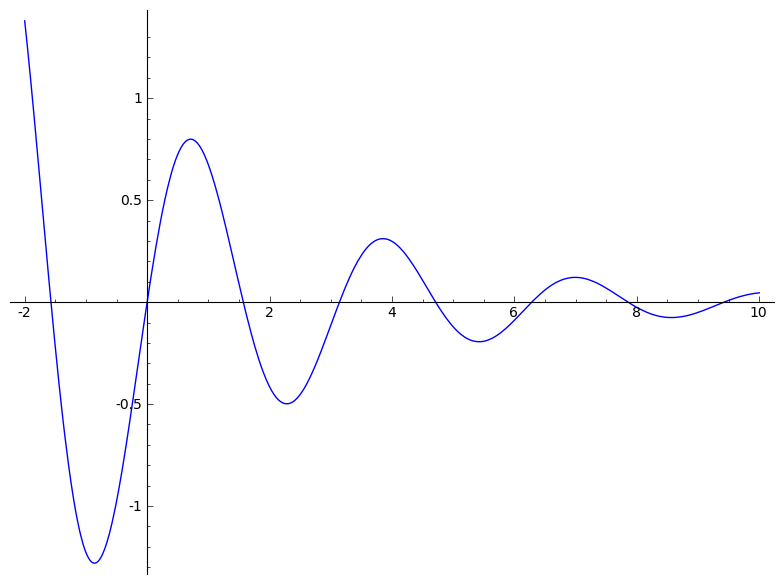
\includegraphics[scale=.1]{imagenes/mu_neg.png} & 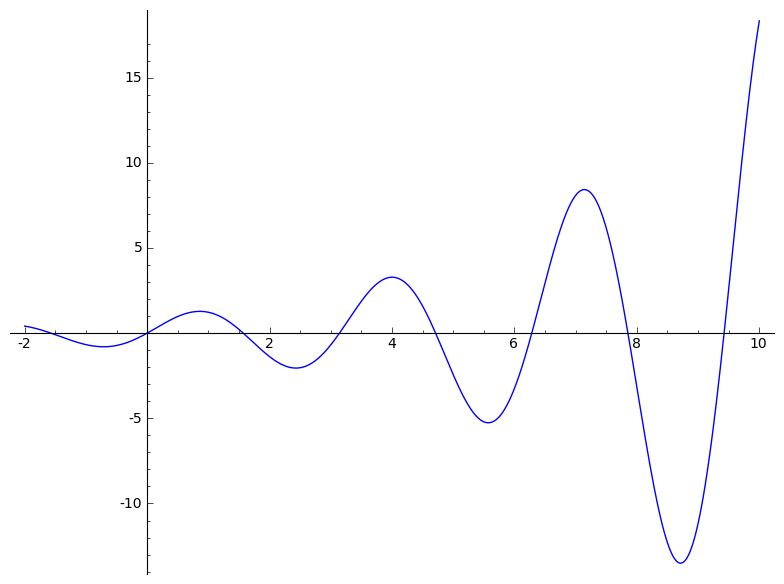
\includegraphics[scale=.1]{imagenes/mu_pos.png}  &
 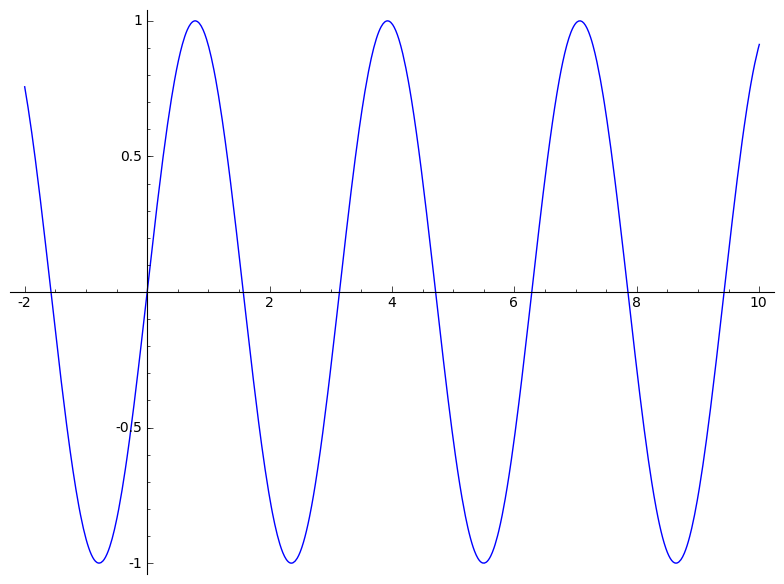
\includegraphics[scale=.1]{imagenes/mu_cero.png}\\
 $\mu<0$ & $\mu>0$ & $\mu=0$\\
\end{tabular}




\end{frame}


\begin{frame}[fragile]{Ecuaciones homogéneas con coeficientes constantes}


3)\textbf{$\boxed{\Delta=p^2-4c=0}$, raices iguales }. Conocemos una solución $\boxed{y_1=e^{-\frac{p}{2}x}}$. Podemos hallar otra
por el método de reducción de orden. Esto consiste en proponer otra solución de la forma $y_2(x)=y_1(x)v(x)$ Dejemos que SAGE nos realice los
cálculos (ver \texttt{uni4b.sage} ).
\begin{sageblock}
x,p=var('x,p')
y=function('y',x)
v=function('v',x)
y1=exp(-p/2*x)
y=v*y1
ecua=y.diff(x,2)+p*y.diff(x)+p^2/4*y==0
ecuav=(ecua/exp(-p/2*x)).simplify_full()
sol=desolve(ecuav,v,ivar=x)
\end{sageblock}
La solución general para $v$ es $v=\sage{sol}$. Así el método mencionado proporciona la solución extra 
\[\boxed{y_2(x)=xe^{-\frac{p}{2}x}}.\]
\end{frame}


\section{Ecuación no homogénea}

\begin{frame}{Ecuaciones no homogéneas. Método coeficientes indeterminados}
\nl \begin{block}{Ecuación no homogénea}
 \boxedeq{\frac{d^2y}{dx^2}+p(x)\frac{dy}{dx}+q(x)y=r(x),}{ec_2_nohom}
donde $p,q,r \in C(I)$ y $r\neq 0$.
 \end{block}

\subsection{Método coeficientes ideterminados}

\nl \begin{block}{Método coeficientes indeterminados}
 
Consiste en buscar soluciones en la misma clase de funciones a la que pertenece $r(x)$. Funciona de manera metódica sólo para algunos tipos de funciones $r(x)$. 
Concretamente para $r(x)$ combinación lineal de funciones polinómicas, exponenciales $e^{\alpha x}$ o trigonométricas $\cos \alpha x$ y $\sen \alpha x$. 
Lo vamos a ilustrar con ejemplos para cada caso.
 \end{block}
 \end{frame}

 
 
 
 
 \defverbatim[colored]\lstI{ 
\begin{lstlisting}
sage: x,p,q,a,A=var('x,p,q,a,A')        
sage: y=function('y',x)
sage: y=A*exp(a*x)     
sage: ecua=y.diff(x,2)+p*y.diff(x)+q*y==exp(a*x)
sage: ecua=(ecua/exp(a*x)).simplify_full()      
sage: ecua
(a^2 + a*p + q)*A == 1
sage: solve(ecua,A)                             
[A == (1/(a^2 + a*p + q))]
\end{lstlisting}
 }
 
 \begin{frame}{Método coeficientes indeterminados. Caso $r(x)=e^{a x}$ y $a^2+pa+q\neq 0$.}
 En esta situación se propone como solución una función de la forma $\boxed{y(x)=Ae^{ax}}$. Usamos SAGE para el cálculos
 
 \lstI
 
 Si $a^2+pa+q\neq 0$,  encontramos la solución particular  $\boxed{y(x)=\frac{1}{(a^2+pa+q)}e^{ax}}$.
 
 
\end{frame}

 
\defverbatim[colored]\lstI{ 
\begin{lstlisting}
sage: x,p,q,a,A=var('x,p,q,a,A')          
sage: y=A*x*exp(a*x)
sage: ecua=y.diff(x,2)+p*y.diff(x)+q*y==exp(a*x)
sage: ecua=(ecua/exp(a*x)).simplify_full()      
sage: ecua
((a^2 + a*p + q)*x + 2*a + p)*A == 1
sage: ecua.subs_expr(a^2 + a*p + q==0)          
(2*a + p)*A == 1

\end{lstlisting}
 }
 \begin{frame}{Método coeficientes indeterminados. Caso $r(x)=e^{a x}$  y $a^2+pa+q= 0$}

En esta situación diremos que la ecuación está en \emph{resonancia}. Más generalmente, diremos que se presenta resonancia cuando $r(x)$ es solución 
del problema homogéneo. 

Propongamos como solución $y(x)=Axe^{ax}$. Hagamos los cálculos con SAGE.

\lstI

Luego, si $2a+p\neq 0$, $\boxed{y(x)=\frac{1}{2a+p}xe^{ax}}$  resuelve el problema.
\end{frame}

\defverbatim[colored]\lstI{ 
\begin{lstlisting}
sage: x,p,q,a,A=var('x,p,q,a,A')               
sage: y=function('y',x)
sage: y=A*x**2*exp(a*x)
sage: ecua=y.diff(x,2)+p*y.diff(x)+q*y==exp(a*x) 
sage: ecua=(ecua/exp(a*x)).simplify_full()      
sage: ecua
((a^2 + a*p + q)*x^2 + 2*(2*a + p)*x + 2)*A == 1
sage: ecua.subs_expr(2*a+p==0,a^2 + a*p + q==0)
2*A == 1

\end{lstlisting}
 }
 
 \begin{frame}{Método coeficientes indeterminados. Caso $r(x)=e^{a x}$, $a^2+pa+q= 0$ y $2a+p=0$}

 Si $2a+p=0$, como también $a^2+pa+q=0$, tenemos que $a$ es una raíz doble de la ecuación $\lambda^2+p\lambda+q=0$. 
 En este caso, proponemos como solución $y(x)=Ax^2e^{ax}$. 
 
 \lstI
 
 Hay que tomar $\boxed{y(x)=\frac{1}{2}x^2e^{ax}}$
 
 
\end{frame}
 
 \defverbatim[colored]\lstI{ 
\begin{lstlisting}
sage: x,p,q,b,A,B=var('x,p,q,b,A,B')             
sage: y=function('y',x)      
sage: y=A*cos(b*x)+B*sin(b*x)
sage: ecua=y.diff(x,2)+p*y.diff(x)+q*y==sin(b*x)
sage: ecua.simplify_full()                      
(b*p*cos(b*x) - (b^2 - q)*sin(b*x))*B - (b*p*sin(b*x) 
...  + (b^2 - q)*cos(b*x))*A == sin(b*x)
sage: ecua=ecua-sin(b*x)                        
sage: ecua
-A*b^2*cos(b*x) - B*b^2*sin(b*x) + (A*cos(b*x) + B*sin(b*x))*q 
...  - (A*b*sin(b*x) - B*b*cos(b*x))*p - sin(b*x) == 0
\end{lstlisting}
 }
 
 
 \begin{frame}{Método coeficientes indeterminados. Caso $r(x)=\sen bx$}
 Proponemos 
 \[y(x)=A\cos x+ B\sen x,\]
 como candidato a solución. 
 
 \lstI
 
 
 
\end{frame}
 
  \defverbatim[colored]\lstI{ 
\begin{lstlisting}
sage: ecua.lhs().coefficient(sin(b*x)).simplify_full()==0
-A*b*p - (b^2 - q)*B - 1 == 0
sage: ecua.lhs().coefficient(cos(b*x)).simplify_full()==0
B*b*p - (b^2 - q)*A == 0
\end{lstlisting}
 }
 
 
 \begin{frame}{Método coeficientes indeterminados. Caso $r(x)=\sen bx$}
La expresión en el miembro de la izquierda es una combinación lineal de las funciones $\cos bx$ y $\sen bx$. Como estas funciones son linealmente independientes
debemos tener que los coeficientes en la combinación lineal deben ser cero
\lstI
Obtenemos un sistema de ecuaciones
\begin{equation}\label{sist_lin_1}
  \left\{\begin{array}{l l}
          -Abp - (b^2 - q)B & = 1\\
          Bbp - (b^2 - q)A &=0
         \end{array}
  \right.
\end{equation}
 
\end{frame}

 \begin{frame}{Método coeficientes indeterminados. Caso $r(x)=\sen bx$}
Para que el sistema tenga solución la matriz de coeficientes debe ser no singular
\[
  0\neq\det \begin{pmatrix}
              -bp & -(b^2-q)\\
              -(b^2-q) & bp
            \end{pmatrix} = -(b^2p^2+(b^2-q)^2)
\]

Podemos suponer $b\neq 0$, de lo contrario la ecuación hubiese sido homogénea. entonces la condición de arriba ocurre si y sólo si 
$p\neq 0$ o $b^2\neq q$. En esa situación encontraremos una solución de la forma
\[
 \boxed{y(x)=A\cos bx + B\sen bx},
\]
donde $A$ y $B$ resuelven \eqref{sist_lin_1}.
\end{frame}



  \begin{frame}{Método coeficientes indeterminados. Caso $r(x)=\sen bx$ con resonancia}\label{eq:forz_res}
Cuando $p=0$ y $b^2= q$ el sistema \eqref{sist_lin_1} puede no tener solución. Notar que en este caso la ecuación queda
\[
 y''+b^2y=\sen bx
\]
Es una ecuación de un oscilador armónico no homogénea. Habíamos visto que justamente $r(x)=\sen bx$ es una solución del problema homogéno. Nuevamente
estamos en una situación de resonancia.  Como en casos anteriores hay que proponer como solución

 \[y(x)=x\left(A\cos x+ B\sen x\right),\]
\end{frame}

 \defverbatim[colored]\lstI{ 
\begin{lstlisting}
sage: x,b,A,B=var('x,b,A,B')        
sage: y=function('y',x)      
sage: y=x*(A*cos(b*x)+B*sin(b*x))
sage: ecua=y.diff(x,2)+b^2*y==sin(b*x)  
sage: ecua=ecua-sin(b*x)    
sage: eql1=ecua.lhs().coefficient(sin(b*x))==0
sage: eql2=ecua.lhs().coefficient(cos(b*x))==0
sage: solve([eql1,eql2],[A,B])
[[A == -1/2/b, B == 0]]
\end{lstlisting}
 }

   \begin{frame}{Método coeficientes indeterminados. Caso $r(x)=\sen bx$ con resonancia}
 \lstI
 
 Encontramos la solución general
 
  \[\boxed{y(x)=-\frac{x}{2b}\cos x}.\]
 
El caso donde $r(x)=\cos bx$ se trata de manera completamente similar.

\end{frame}





 \defverbatim[colored]\lstI{ 
\begin{lstlisting}
sage: PoliQX=QQ['X']
sage: print(PoliQX) 
Univariate Polynomial Ring in X over Rational Field
sage: PoliRX=RR['X'] 
sage: print(PoliRX) 
Univariate Polynomial Ring in X over Real Field with 53 bits of 
...precision
sage: PoliZ3X=Integers(3)['X']
sage: print(PoliZ3X)
Univariate Polynomial Ring in X over Ring of integers modulo 3
sage: p=PoliZ3X([1,1,1])
sage: p
X^2 + X + 1
sage: p+p
2*X^2 + 2*X + 2
sage: p+p+p
0
sage: PoliZ3Xb = PolynomialRing(Integers(3),"X")
sage: PoliZ3X is PoliZ3Xb  
True
sage: X+X    
NameError: name 'X' is not defined
sage: PoliZ3Xc.<X> = Integers(3)["X"]
sage: PoliZ3Xc([1,2,1])+X
X^2 + 1


\end{lstlisting}
 }

   \begin{frame}{Disgresión: \href{http://www.sagemath.org/doc/tutorial/tour_polynomial.html}{anillos de polinomios en SAGE}. Definiendo un anillo de polinomios sobre $\mathbb{Q}$}

\lstI


\end{frame}


 \defverbatim[colored]\lstI{ 
\begin{lstlisting}
sage: P.<X,Y>=QQ["X,Y"]                    
sage: 1+X+X^2+Y^3 in P 
True
sage: p=sum([j*X^j*Y^(3-j) for j in range(4)] )
sage: p in P
True
sage: p
3*X^3 + 2*X^2*Y + X*Y^2
sage: P=QQ[['a'+str(j) for j in range(8)]]
sage: P
Multivariate Power Series Ring in a0, a1, a2, a3, a4,
...a5, a6, a7 over Rational Field
sage: a0 in P
NameError: name 'a0' is not defined
sage: a=P.gens()                          
sage: a
(a0, a1, a2, a3, a4, a5, a6, a7)
sage: a[0] in P
True
sage: type(a[0])
<class 'sage.rings.multi_power_series_ring_element.
...MPowerSeriesRing_generic_with_category.element_class'>
sage: sum([a[j]*j for j in range(8)])
a1 + 2*a2 + 3*a3 + 4*a4 + 5*a5 + 6*a6 + 7*a7
sage: sum([a[j]*j for j in range(8)]) in P
True



\end{lstlisting}
 }

   \begin{frame}{Anillo de polinomios en varias variables}

\lstI


\end{frame}




 \defverbatim[colored]\lstI{ 
\begin{lstlisting}
sage: A=QQ[['a'+str(j) for j in range(5)]]
sage: A
Multivariate Power Series Ring in a0, a1, a2, a3, a4 
....over Rational Field
sage: P.<X>=A["X"]
sage: a=A.gens()
sage: a
(a0, a1, a2, a3, a4)
sage: a[0]*X+a[1]*X^2 in P
True
sage: a[0]*X+a[1]*X^2     
a1*X^2 + a0*X
sage: (a[0]*X+a[1]*X^2)^2 
a1^2*X^4 + 2*a0*a1*X^3 + a0^2*X^2
sage: p=sum([a[j]*X^j for j in range(5)])
sage: p
a4*X^4 + a3*X^3 + a2*X^2 + a1*X + a0




\end{lstlisting}
 }

   \begin{frame}{Anillo de polinomios sobre anillo de polinomios}

\lstI


\end{frame}



 \defverbatim[colored]\lstI{ 
\begin{lstlisting}
sage: grado=4
sage: lista_var=['a'+str(j) for j in range(grado)] 
sage: lista_var+=['b'+str(j) for j in range(grado)]
sage: lista_var+=['p', 'q']                        
sage: A = PolynomialRing(QQ,lista_var)
sage: P=A['X']
sage: r=P([A.gen(i) for i in range(grado)])
sage: r
a3*X^3 + a2*X^2 + a1*X + a0
sage: y=P([A.gen(i) for i in range(grado,2*grado)])
sage: y
b3*X^3 + b2*X^2 + b1*X + b0
sage: eq=y.derivative(2)+y.derivative()*A.gen(2*grado)+y*A.gen(2*grado+1)-r
sage: ecuaciones=[SR(l)==0 for l in eq.coefficients()]
sage: parametros=[SR(A.gen(j)) for j in range(2*grado+2)] 
sage: Sol=solve(ecuaciones,parametros[grado:2*grado])
sage: show(Sol[0])
\end{lstlisting}
 }

\begin{frame}{Método coeficientes indeterminados. Caso $r(x)$ polinomio}
 
Hay que proponer como solución un polinomio, en primera instancia, del mismo grado. Invocando SAGE.

\lstI

\end{frame}

\begin{frame}{Método coeficientes indeterminados. Caso $r(x)$ polinomio}
Encontramos las soluciones

\[
  \begin{split}
      b_{0} &= \frac{a_{0} q^{3} - 6 \, a_{3} p^{3} - {\left(a_{1} p + 2 \, a_{2}\right)} q^{2} + 2 \, {\left(a_{2} p^{2} + 6 \, a_{3} p\right)} q}{q^{4}},\\
      b_{1} &= \frac{a_{1} q^{2} + 6 \, a_{3} p^{2} - 2 \, {\left(a_{2} p + 3 \, a_{3}\right)} q}{q^{3}},\\
      b_{2} &= \frac{a_{2} q - 3 \, a_{3} p}{q^{2}},\\
      b_{3} &= \frac{a_{3}}{q}
  \end{split}
\]
que tienen sentido solo cuando $q\neq 0$.
\end{frame}

\begin{frame}{Método coeficientes indeterminados. Caso $r(x)$ polinomio y resonancia}
El caso $q=0$ es una forma de resonancia. Puede ser tratado como las anteriores resonancias, pero notando que la ecuación se reduce a $y''+py'=r$ conviene 
tomar $v=y'$ como
nueva variable dependiente y reducir la ecuación a una de primer orden.

Por último señalemos que si deseamos resolver un problema de la forma
\[L[y]\equiv y''+py'+qy=r_1(x)+\cdots +r_n(x),\]
donde las funciones $r_i$ son de alguna de las formas descriptas en los casos previos,
entonces la linealidad de $L$ implica que, si $y_i$ 
resuelve $L[y_i]=r_i$, $y=y_1+\cdots +y_n$ resuelve la ecuación deseada. 

\end{frame}

\subsection{Método de variación de los parámetros}

\begin{frame}{Método variación de los parámetros}
Queremos resolver la ecuación
\begin{equation}\label{eq:2orden_gen}
  y''(x)+p(x)y'(x)+q(x)y(x)=r(x).
\end{equation}
Supongamos que contamos con un par de soluciones $y_1$, $y_2$ linealmente independientes de la ecuación homogénea asociada 
\begin{equation}\label{eq:hom_asoc}
  y''(x)+p(x)y'(x)+q(x)y(x)=0.
\end{equation}

El método de \href{http://en.wikipedia.org/wiki/Variation_of_parameters}{variacion de los parámetros} consiste en proponer una solución de la forma
\boxedeq{y(x)=c_1(x)y_1(x)+c_2(x)y_2(x).}{eq:var_param0}

\end{frame}



\begin{frame}{Método variación de los parámetros}

Hay dos funciones incognitas $c_1$ y $c_2$, pero sólo una ecuación. Tendremos por esto libertad de introducir otra condición que consideremos conveniente.

Tenemos
\[
  y'=c_1'y_1+c_1y_1'+c_2'y_2+c_2y_2'.
\]
Pidamos que
\begin{equation}\label{eq:var_param1}
 c_1'y_1+c_2'y_2=0.
\end{equation}
Supuesta esta igualad
\[ y'= c_1y_1'+c_2y_2'.\]
Derivando
\[ y''= c_1'y_1'+c_2'y_2'+c_1y_1''+c_2y_2''.\]


\end{frame}
\begin{frame}{Método variación de los parámetros}

Entonces
\[
 \begin{split}
    r(x)&=y''+py'+qy\\
    &=c_1'y_1'+c_2'y_2'+c_1y_1''+c_2y_2''+p(c_1y_1'+c_2y_2')+q(c_1y_1+c_2y_2)\\
    &=c_1(y_1''+py_1'+qy_1)+c_2(y_2''+py_2'+qy_2)+c_1'y_1'+c_2y_2'\\
    &=c_1'y_1'+c_2'y_2'
 \end{split}
\]
Esta ecuación junto a \eqref{eq:var_param1} nos dan el sistema
\boxedeq{
  \left\{\begin{array}{c c}
            c_1'y_1+c_2'y_2&=0\\
            c_1'y_1'+c_2'y_2'&=r
         \end{array}
  \right. 
}{eq:var_param_sis}
Las incognitas son $c_1'$ y $c_2'$. El determinante de la matriz de coeficientes es precisamente el Wronskiano $W$ de las soluciones $y_1$ e $y_2$, por la suposición
de independencia $W\neq 0$ y por lo tanto el sistema tiene solución única.


\end{frame}

\begin{frame}{Método variación de los parámetros}
Se tiene
\[c_1'=-\frac{\det\begin{pmatrix}
                0 & y_2\\
                r & y_2'
               \end{pmatrix}
}{W}=-\frac{ry_2}{W}
\]
y
\[c_2'=-\frac{\det\begin{pmatrix}
                y_1 & 0\\
                y_1' & r
               \end{pmatrix}
}{W}=\frac{ry_1}{W}
\]
\end{frame}

\begin{frame}{Método variación de los parámetros}
En consecuencia
\boxedeq{c_1=-\int\frac{ry_2}{W}dx}{eq:c1}
y
\boxedeq{c_2=\int\frac{ry_1}{W}}{eq:c2}

Usando estas fórmulas y \eqref{eq:var_param0} obtenemos una solución particular del sistema. La solución general es la suma de la particular más
una solución general del homogéneo. Esta última solución general se escribe como una combinación lineal genérica entre $y_1$ e $y_2$.
\end{frame}
 \defverbatim[colored]\lstI{ 
\begin{lstlisting}
sage: x=var('x')
sage: y1=sin(x)
sage: y2=cos(x)
sage: W=y1*y2.diff()-y1.diff()*y2
sage: W.simplify_full() #chequeamos independencia
-1
sage: r=csc(x)
sage: y=(r*y1/W).integral(x)*y2-(r*y2/W).integral(x)*y1 #formula
sage: y
-x*cos(x) + log(sin(x))*sin(x)
sage: c1,c2=var('c1,c2')
sage: z=y+c1*y1+c2*y2 #solucion general
sage: (z.diff(x,2)+z-r).simplify_trig()
0
sage: #resolvemos pvi
sage: C=solve([z(x=pi/2)==0,z.diff(x).subs(x=pi/2)==1],[c1,c2])
sage: C
[[c1 == 0, c2 == 1/2*pi - 1]]
sage: A,B=C[0]
sage: y=z.subs_expr(A,B)
sage: y
1/2*(pi - 2)*cos(x) - x*cos(x) + log(sin(x))*sin(x)
sage: y(x=pi/2)
0
sage: y.diff()(x=pi/2)
1

\end{lstlisting}
 }

\begin{frame}{Método variación de los parámetros}
\textbf{Ejemlo} Resolver el siguiente pvi $y''+y=\csc x$, $y\left(\tfrac{\pi}{2}\right)=0$ y  $y'\left(\tfrac{\pi}{2}\right)=1$.
\lstI
\end{frame}

\section{Conclusiones}

\begin{frame}{Conclusiones}
\begin{enumerate}
 \item Si podemos encontrar dos soluciones linealmente independientes de una ecuación lineal homogénea de segundo orden, tenemos la solución general a traves de 
 combinaciones lineales.
 \item Si tenemos una solución no trivial de una ecuación lineal homogénea de segundo orden podemos hallar otra por el método de reducción de orden.
 \item Podemos resolver completamente una ecuación lineal homogénea de segundo orden con coeficientes constantes.
 \item Podemos resolver algunos problemas no homogéneos por el método de coeficientes indeterminados.
 \item Si conocemos las soluciones del problema homogéneo podemos resolver, en teoría, el no homogéneno para cualquier $r(x)$ por el método de variación 
 de los parámetros
\end{enumerate}

\end{frame}

\section{Aplicaciones}

\begin{frame}{Aplicaciones. Vibraciones mecánicas }
 
\textbf{Problema:} Estudiar el movimiento de un resorte (cómo el de la unidad anterior) pero suponer que además de actuar sobre la masa la fuerza elástica del resorte,
tenemos una fuerza de fricción debida ala resistencia del medio. Por la acción de esta fuerza, se dice que es un sistema resorte-masa amortiguado.
Además suponemos que hay otra fuerza $F$ externa y que sólo depende de $t$. Por ejemplo si el resorte se colocase verticalmente y se dejase suspendida 
la masa, $F$ sería la fuerza de gravedad. Si la masa estuviese hecha de metal, $F$ podría ser una fuerza provista por un imán. Por la acción de esta fuerza el sistema se 
dice forzado. Por consiguiente el sistema completo, con la acción de las tres fuerzas, se denomina un sistema resorte-masa, amortiguado y forzado.
\end{frame}

\begin{frame}{Aplicaciones. Vibraciones mecánicas }

La fuerza elástica del resorte se modeliza con la Ley de Hooke. 
Para la amortiguación, supongamos que su módulo  es proporcional a la velocidad de la masa. La constante de proporcionalidad $c$ se llama coeficiente de 
\href{http://es.wikipedia.org/wiki/Viscosidad}{viscosidad}. La dirección y sentido de la fuerza amortiguadora es siempre contraria 
al movimiento. Por el principio de conservación de la energía, vemos que la fuerza de amortiguación siempre realiza un trabajo $W$ negativo, por consiguiente
hace perder energía cinética. De la fuerza externa $F$ no sabemos nada en principio. Por todo lo expuesto, si ponemos un sistema 
de coordenadas con origen en la posición de equilibrio del sistema masa-resorte y si $x(t)$ es la posición de la masa en el momento $t$, la ecuación que gobierna 
el sistema masa-resorte con amortiguación y forzamiento es 

\boxedeq{mx''(t)\underbrace{=}_\text{2° Ley Newton}\underbrace{-kx(t)}_
\text{Hooke}\underbrace{-cx'(t)}_\text{Amortiguación}+\underbrace{F(t)}_\text{Fuerza externa}}{eq:res_amor_for}

\end{frame}

\begin{frame}{ Vibraciones amortiguadas no forzadas ($c>0$, $F=0$) }
 
Escribamos la ecuación \eqref{eq:res_amor_for} de la siguiente froma

\begin{equation}\label{eq:res_amor}
  \boxed{x''(t)+2\mu x'(t)+\omega^2x=0}\quad \mu:=\frac{c}{2m},\omega:=\sqrt{\frac{k}{m}}. 
\end{equation}

Las raíces de la ecuación característica son
\[
 \boxed{\lambda_{1,2}=-\mu\pm\sqrt{\Delta},\quad \Delta:=\mu^2-\omega^2}
\]

\textbf{Caso $\Delta>0$.} Aquí la viscocidad es ``grande'' relativa ala rigidez $k$. Se dice que el sistema está sobreamortiguado. En este caso tenemos dos soluciones
linealmente independientes y la solución general es de la forma
\[x(t)=c_1e^{\lambda_1t}+c_2e^{\lambda_2t}\]
Notar que $\lambda_1,\lambda_2<0$.
\end{frame}



\defverbatim[colored]\lstI{ 
\begin{lstlisting}
sage: lambda1,lambda2=var('lambda1,lambda2')
sage: t=var('t')
sage: x=c1*e^(lambda1*t)+c2*e^(lambda2*t)
sage: x0=var('x0')
sage: C=solve([x(t=0)==x0,x.diff(t).subs(t=0)==0],
....[c1,c2],solution_dict=True)
sage: C
[{c2: lambda1*x0/(lambda1 - lambda2), c1: -lambda2*x0/(lambda1 - lambda2)}]
sage: x=x.subs(C[0])
sage: x.show()
sage: latex(x)
-\frac{\lambda_{2} x_{0} e^{\left(\lambda_{1} t\right)}}{\lambda_{1} - \lambda_{2}} + 
...\frac{\lambda_{1} x_{0} e^{\left(\lambda_{2} t\right)}}{\lambda_{1} - \lambda_{2}}



\end{lstlisting}
 }
\begin{frame}{ Vibraciones amortiguadas no forzadas ($c>0$, $F=0$) }
Supongamos que el sistema masa-resorte parte del resposo $x'(0)=0$ y de una posición indeterminada $x_0$. Resolvamos este pvi
\lstI

\boxedeq{
  x(t)= x_0\left\{ \frac{\lambda_{1}  
  e^{\lambda_{2} t}}{\lambda_{1} - \lambda_{2}}-\frac{\lambda_{2} e^{\lambda_{1} t}}{\lambda_{1} - \lambda_{2}}\right\}
}{eq:sol_sub_amor}
\end{frame}



\defverbatim[colored]\lstI{ 
\begin{lstlisting}
sage: x=x.subs({lambda1:-1,lambda2:-2,x0:1})
sage: x.plot((x,0,10))

\end{lstlisting}
 }

\begin{frame}{ Vibraciones amortiguadas no forzadas ($c>0$, $F=0$) }
La masa podría haber pasado por la posición de equilibrio sólo en el pasado puesto que $x(t)=0$ cuando
\[\boxed{t=\frac{1}{\lambda_1-\lambda_2}\ln\frac{\lambda_1}{\lambda_2}<0}\]
 
 \lstI 
 
 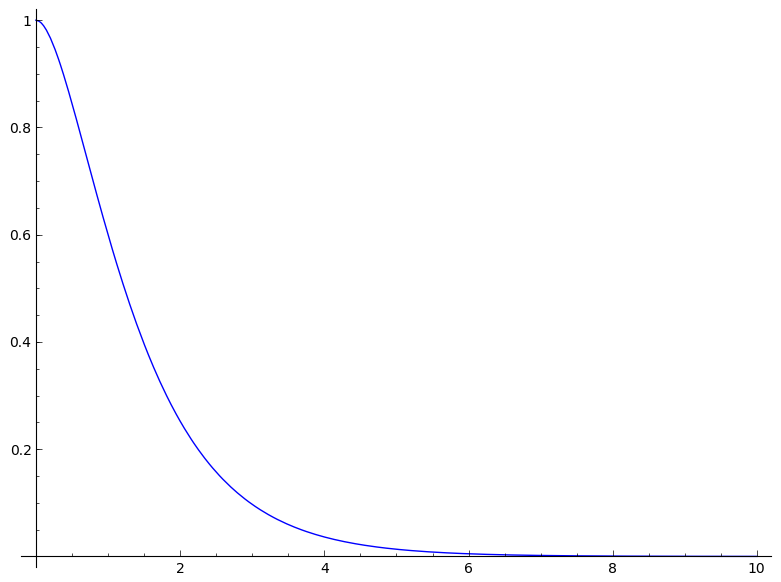
\includegraphics[scale=.2]{imagenes/sobreamortiguado.png}


\end{frame}


\begin{frame}{ Vibraciones amortiguadas no forzadas ($c>0$, $F=0$) }

\begin{center}

\begin{figure}[h]
\animategraphics[controls, scale=.4]{15}{res_sobre/res_sobre-}{0}{60}
\vspace{.5cm}
\caption{Masa-resorte sobreamortiguado}
\end{figure}
\end{center}
\end{frame}



\defverbatim[colored]\lstI{ 
\begin{lstlisting}
sage: c1,c2=var('c1,c2')
sage: mu=var('mu')
sage: t=var('t')
sage: x=e^(-mu*t)*(c1+c2*t)
sage: x0=var('x0')
sage: C=solve([x(t=0)==x0,x.diff(t).subs(t=0)==0],[c1,c2],solution_dict=True)
sage: C
[{c2: mu*x0, c1: x0}]
sage: x=x.subs(C[0]).subs({mu:.1,x0:1})
sage: x.plot((x,0,100))

\end{lstlisting}
 }



\begin{frame}{ Vibraciones amortiguadas no forzadas ($c>0$, $F=0$) }
\textbf{Caso $\Delta=0$.} En esta situación se dice que hay amortiguación crítica. Las raíces son iguales $\lambda_1=\lambda_2=-\mu$. Sabemos que
\boxedeq{x_1(t)=c_1e^{-\mu t}+c_2te^{-\mu t}=e^{-\mu t}\{c_1+c_2t\}}{eq:sol_gen_crit}
 \lstI 
 \begin{center}
   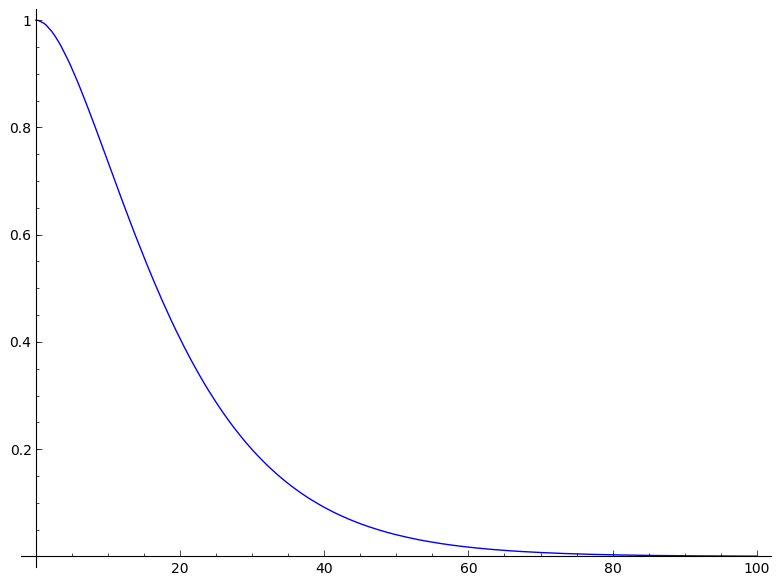
\includegraphics[scale=.1]{imagenes/crit_amortiguado.png}
 \end{center}


 


\end{frame}

\defverbatim[colored]\lstI{ 
\begin{lstlisting}
sage: c1,c2=var('c1,c2')
sage: mu=var('mu')
sage: nu=var('nu')
sage: x0=var('x0')
sage: x=e^(-mu*t)*(c1*cos(nu*t)+c2*sin(nu*t))
sage: t=var('t')
sage: C=solve([x(t=0)==x0,x.diff(t).subs(t=0)==0],[c1,c2],solution_dict=True)
sage: x=x.subs(C[0]).subs({mu:.1,nu:4,x0:1})
sage: x.plot((x,0,100))


\end{lstlisting}
 }
\begin{frame}{ Vibraciones amortiguadas no forzadas ($c>0$, $F=0$) }
\textbf{Caso $\Delta<0$.} Caso subamortiguado, $\lambda_{1,2}=-\mu\pm\nu i$ con $\nu=\sqrt{|\Delta|}=\sqrt{|\omega^2-\mu^2|}$.
La solución general viene dada por

\boxedeq{x(t)=e^{-\mu t}\left\{ c_1\cos \nu t+c_2\sen \nu t    \right\}}{eq:sol_gen_sub}
 \lstI 
 \begin{center}
   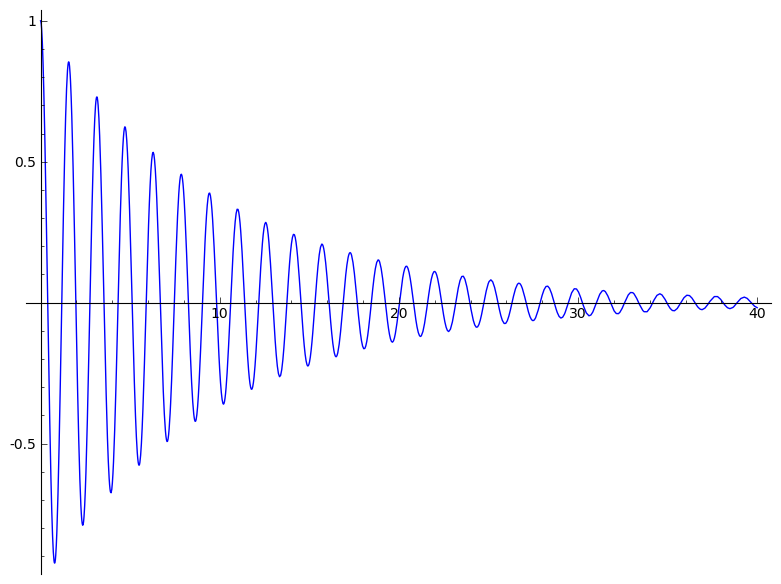
\includegraphics[scale=.1]{imagenes/subamortiguado.png}
 \end{center}
 


\end{frame}
 


\begin{frame}{ Vibraciones amortiguadas no forzadas ($c>0$, $F=0$) }
\begin{figure}[h]
%\animategraphics[controls, scale=.4]{15}{res_sub/res_sub-}{0}{60}
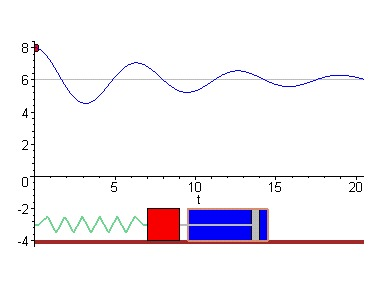
\includegraphics[scale=.4]{res_sub/res_sub-0.jpg}
\vspace{.5cm}
\caption{Masa-resorte subamortiguado}
\end{figure}
 
\end{frame}


\begin{frame}{ Vibraciones amortiguadas no forzadas ($c>0$, $F=0$) }
Se suele escribir la ecuación \eqref{eq:sol_gen_sub} de otra forma. Expresemos el vector $(c_1,c_2)$ en 
coordenadas polares. 
\[
c_1=\rho\cos\alpha,\quad c_2=\rho\sen\alpha.
\]
Entonces
\[
 x(t)=e^{-\mu t}\left\{ c_1\cos \nu t+c_2\sen \nu t    \right\}=\boxed{\rho e^{-\mu t}\cos(\nu t-\alpha)}.
\]
Llamaremos este régimen \emph{movimiento  cuasi-oscilatorio}. Se ejecutan vibraciones que se van amortiguando
de \href{http://es.wikipedia.org/wiki/Frecuencia}{frecuencia}
\[
  f=\frac{1}{\text{período}}=\frac{\nu}{2\pi},\quad \nu=\sqrt{\omega^2-\mu^2}=\sqrt{\left(\frac{k}{m}\right)^2-
  \left(\frac{c}{2m}\right)^2}.
\]
En lugar de la frecuencia se suele considerar la 
\href{http://luz.izt.uam.mx/mediawiki/index.php/Frecuencia_angular}{frecuencia angular} que se define como 
$2\pi f$. La ventaja de esta definición es que la frecuencia ángular de la función de arriba es
$\nu$. 
\end{frame}



\begin{frame}{ Vibraciones amortiguadas no forzadas ($c>0$, $F=0$) }
\textbf{Ejercicio:} En cualquiera de las situaciones descriptas, $x(t)\to 0$ y $x'(t)\to 0$, cuando $t\to\infty$. 
Es decir, la masa se va deteniendo.                                                                                                                                                                                                                                                                         
 


\end{frame}


\begin{frame}{ Vibraciones no amortiguadas y forzadas ($c=0$, $F\neq 0$) }
Vamos a considerar una fuerza externa oscilatoria de frecuencia angular $\omega_0$ y amplitud $F_0$. Tenemos que resolver
\boxedeq{x''(t)+\omega^2 x(t)=F_0\cos(\omega_0 t).}{eq:ecua_2orden_nohom}
Usaremos el método de coeficientes indeterminados y SAGE. Antes, recordar que si $\omega=\omega_0$ estamos en 
resonancia. Tendremos que considerar ese caso por separado. Supongamos pues $\omega\neq\omega_0$.

El siguiente código se puede encontrar en la carpeta \texttt{scripts} del repositorio 
\href{https://github.com/fdmazzone/Ecuaciones_Diferenciales}{GitHub} de esta  materia. El script se denomina \texttt{osc\_arm\_forz\_noamort.sage} 
 

\end{frame}



\begin{frame}{ Vibraciones no amortiguadas y forzadas ($c=0$, $F\neq 0$) }
 \lstinputlisting{scripts/osc_arm_forz_noamort.sage}

 
Notar que el determinante del sistema de ecuaciones algebraicas es $-(\omega-\omega_0)^2$. Luego la matriz 
es no singular sólo en no resonancia. 

La solución general del problema es la solución particular que acabamos de obtener más una solución 
general del homogéneo que sabemos es una combinación lineal generica entre $\cos \omega t$ y $\sin \omega t$.


 
 
\end{frame}

\begin{frame}{ Vibraciones no amortiguadas y forzadas ($c=0$, $F\neq 0$) }
\boxedeq{x(t)=\frac{F_{0} \cos\left(\omega_{0} t\right)}{\omega^{2} - \omega_{0}^{2}}+
c_1\cos(\omega t)+c_2\sin(\omega t).}{eq:sol_gen_noamort_forz}

Como ya hemos visto, considerando las coordenadas polares $\rho$ y $\alpha$ de $c_1,c_2)$
podemos reescribir la solución 


\[x(t)=\frac{F_{0} \cos\left(\omega_{0} t\right)}{\omega^{2} - \omega_{0}^{2}}+
\rho\cos(\omega t-\alpha)
\]

Vemos que el movimiento es la superposición de dos movimientos oscilatorios de frecuencias $\omega$, que se
denomina la \emph{frecuencia natural} del resorte, y $\omega_0$ que se denomina \emph{frecuencia impresa}.
 
\end{frame}

\defverbatim[colored]\lstI{ 
\begin{lstlisting}
sage: t,omega,omega0,F0,rho,alpha=var('t,omega,omega0,F0,rho,alpha')
sage: x=F0/(omega^2-omega0^2)*cos(omega0*t)+rho*cos(omega*t-alpha)  
sage: assume(-pi<alpha, alpha<2*pi)
sage: solve([x(t=0)==0,x.diff(t).subs(t=0)==0],[rho,alpha])         
[omega*rho*sin(alpha) == 0, rho*cos(alpha) + F0/(omega^2 - omega0^2) == 0]
sage: x0=x(alpha=0)
sage: sol=solve([x0(t=0)==0,x0.diff(t).subs(t=0)==0],rho,\
solution_dict=True) 
sage: x0=x0.subs(sol[0])
sage: x0.factor().show()

\end{lstlisting}
 }


\begin{frame}{ Vibraciones no amortiguadas y forzadas ($c=0$, $F\neq 0$) }
Resolvamos el pvi
\[
 \left\{\begin{array}{l}
         x''(t)+\omega^2x(t)=F_0\cos(\omega_0 t),\\
         x'(0)=x(0)=0\\
        \end{array}
\right.
\]


\lstI

\[x(t)=-\frac{F_{0} \cos\left(\omega t\right)}{\omega^{2} - \omega_{0}^{2}} + \frac{F_{0} \cos\left(\omega_{0} t\right)}{\omega^{2} - \omega_{0}^{2}}
\]
\end{frame}

\defverbatim[colored]\lstI{ 
\begin{lstlisting}
sage: x1=x0.subs({F0:1,omega:1,omega0:.9}) 
sage: x1.plot(x,0,200)
\end{lstlisting}
 }


\begin{frame}{ Vibraciones no amortiguadas y forzadas ($c=0$, $F\neq 0$) }
Ahora usemos la identidad $\cos(a-b)-cos(a+b)=2\sen a\sen b$, con $a=\frac12 (\omega+\omega_0)$ y
$b=\frac12 (\omega-\omega_0)$. Deducimos
\boxedeq{%
  x(t)=\frac{2F_{0} }{\omega^{2} - \omega_{0}^{2}}\sen (\omega-\omega_0)t \sen (\omega+\omega_0)t. 
}{eq:sol_gen_pulsos}
Esta  expresión la podemos ver como una onda de frecuencia  grande $\omega+\omega_0$ modulada por una de frecuencia 
chica $\omega-\omega_0$. 
\lstI
\begin{center}
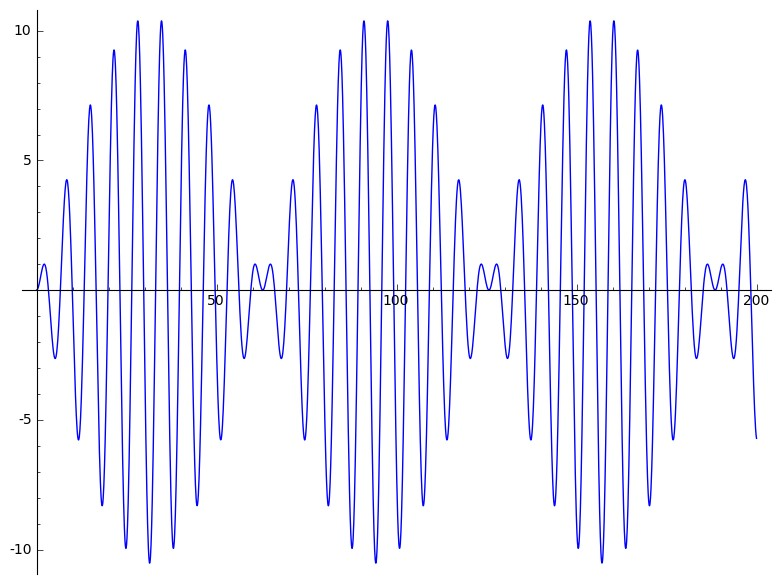
\includegraphics[scale=.15]{imagenes/batido.jpg}
\end{center}


\end{frame}
\defverbatim[colored]\lstI{ 
\begin{lstlisting}
sage: limit(x0,omega0=omega)
1/2*F0*t*sin(omega*t)/omega
\end{lstlisting}
 }

\begin{frame}{ Vibraciones no amortiguadas y forzadas ($c>0$, $F\neq 0$) }
Calculemos el límite $\lim_{\omega_0\to\omega}x(t)$,
\lstI

\[x(t)=\frac{F_{0} t \sin\left(\omega t\right)}{2 \, \omega}
\]
El caso $\omega=\omega_0$ es el caso con resonancia, que debemos resolver como fue indicado en la página \ref{eq:forz_res}, 
esto es proponiendo como solución $y(x)=x\left(A\cos x+ B\sen x\right)$. El siguiente código sage muestra que la solución es la misma función
que la obtenida por el proceso de límite de los casos sin resonancia.

\lstinputlisting{scripts/osc_arm_forz_noamort_res.sage}

\end{frame}

 \begin{frame}{ Vibraciones no amortiguadas y forzadas ($c>0$, $F\neq 0$) } 
Se producen ``vibraciones'' no acotadas.
\begin{center}
 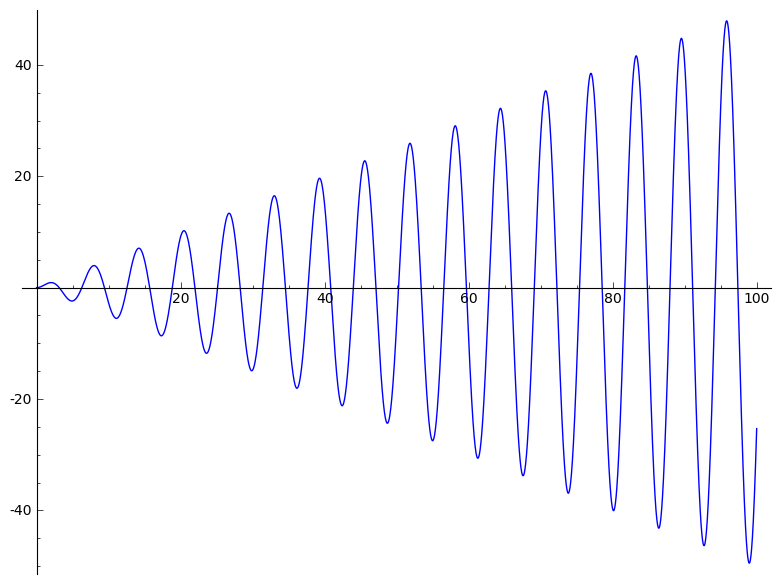
\includegraphics[scale=0.3]{imagenes/osc_arm_forz_res.png}
\end{center}

Ver la notebook \texttt{batido.sws}. En la wiki \href{http://wiki.sagemath.org/interact/misc\#Hearing_a_trigonometric_identity}{Hearing a trigonometric identity}
se puede escuchar ondas sonoras con los fenómenos de resonancia y batido.

\end{frame}



\begin{frame}{ Vibraciones amortiguadas y forzadas ($c>0$, $F\neq 0$) }
Vamos a considerar una fuerza externa oscilatoria de frecuencia $\omega_0$ y amplitud $F_0$. Tenemos que resolver
\boxedeq{x''(t)+2\mu x'(t)+\omega^2 x(t)=F_0\cos(\omega_0 t).}{eq:ecua_2orden_amort_nohom}
\lstinputlisting{scripts/osc_arm_forz_amort.sage}


\end{frame}



\defverbatim[colored]\lstI{ 
\begin{lstlisting}
sage: rho=sqrt(A**2+B**2).subs(SolAB[0]).simplify_full()                                         
sage: show(rho)
\end{lstlisting}
 }


 
\begin{frame}{ Vibraciones amortiguadas y forzadas ($c>0$, $F\neq 0$) } 
\boxedeq{x(t)=
  \frac{2 \, F_{0} \mu \omega_{0} \sin\left(\omega_{0} t\right)}{\omega^{4} + \omega_{0}^{4} + 2 \,
  {\left(2 \, \mu^{2} - \omega^{2}\right)} \omega_{0}^{2}} + \frac{{\left(F_{0} \omega^{2} - 
  F_{0} \omega_{0}^{2}\right)} \cos\left(\omega_{0} t\right)}{\omega^{4} + 
  \omega_{0}^{4} + 2 \, {\left(2 \, \mu^{2} - \omega^{2}\right)} \omega_{0}^{2}}
}{eq:SolGennoHom}


Es un movimiento oscilatorio de frecuencia angular $\omega_0$. Podemos escribir $x(t)=\rho\cos(\omega_0 t-\alpha)$, 
donde $(\rho,\alpha)$ son las coordenadas polares de $(A,B)$. En particular $\rho=\sqrt{A^2+B^2}$
Recurrimos nuevamente a SAGE
\lstI
\[
\rho(\omega_0)=\frac{F_{0}}{\sqrt{\omega^{4} + \omega_{0}^{4} + 2 \, {\left(2 \, \mu^{2} - \omega^{2}\right)} \omega_{0}^{2}}}=
\frac{F_{0}}{\sqrt{(\omega^2-\omega_0^2)^2+4\mu^2\omega_0^2}}
\]
\end{frame}

\defverbatim[colored]\lstI{ 
\begin{lstlisting}
sage: plot(rho.subs({F0:1, mu:.1,omega:5},(omega0,0,10) )
\end{lstlisting}
 }



\begin{frame}{ Vibraciones amortiguadas y forzadas ($c>0$, $F\neq 0$) } 
\[\alpha=\atan2\left(  {{\omega^{2} - 
  \omega_{0}^{2}} }  ,  {2 \,  \mu \omega_{0} }   \right)
\]
En una consola de sage entrar \texttt{atan2?} para averiguar que función es $\atan2$. 

Grafiquemos la función $\rho(\omega_0)$ para $\omega=5$ y $\mu=0.1$. 

\lstI 
\begin{center}
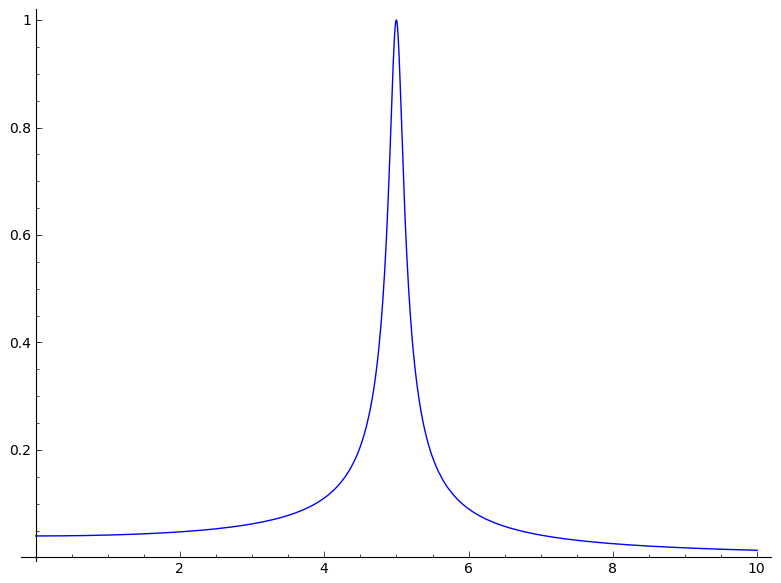
\includegraphics[scale=.2]{imagenes/rho_graf.png}
\end{center}

\end{frame}




 \defverbatim[colored]\lstI{ 
\begin{lstlisting}
sage: sol=solve(rho.diff(omega0),omega0)
sage: sol
[omega0 == -sqrt(-2*mu^2 + omega^2), omega0 == sqrt(-2*mu^2 + omega^2), omega0 == 0]
sage: rho.diff(omega0,2).subs(sol[1]).simplify_full().show()
\end{lstlisting}
 }
 \defverbatim[colored]\lstII{ 
\begin{lstlisting}
sage: sol[1].rhs().subs({mu:.1,omega:5})                         
4.99799959983992
\end{lstlisting}
 } 
 \begin{frame}{ Vibraciones amortiguadas y forzadas ($c>0$, $F\neq 0$) } 
La función tiene un notorio máximo  cerca de $\omega_0=5$. Seguramente es debido a la aparición de resonancias. Hallemos el punto de máximo exacto. 
\lstI
Si $2\mu^2<\omega$ tendremos un máximo (en realidad un máximo local) en  $\omega_{0} = \sqrt{-2 \, \mu^{2} + \omega^{2}}$. En el ejemplo que graficamos
el máximo ocurre en
\lstII
Vale decir, un oscilador armónico en reposo es más sensible a exitaciones en ciertas frecuencias, aproximadamente la frecuencia
natural del resorte cuando el coeficiente de viscocidad $c=2m\mu$ es chico. Esto es utilizado para diseñar dispositivos que captan ondas sísmicas.


\end{frame}

 \begin{frame}{ Vibraciones amortiguadas y forzadas ($c>0$, $F\neq 0$) } 
 Hasta aquí hemos encontrado una solución particular del sistema no homogéneo. Para encontrar una solución general deberíamos adicionar a la particular que disponemos
 una solución general $x_g(t)$  de la ecuación homogénea.  La forma de esta solución general es de alguno de los tipos \ref{eq:sol_gen_sub},
 \ref{eq:sol_gen_crit} o \ref{eq:sol_sub_amor}. Sin embargo no nos importa ahora la fórmula explícita de estas soluciones, sino que nos interesa resaltar que 
 tratese del tipo que se trate, se satisface que $\lim_{t\to\infty}x_g(t)=0$. Por este motivo, vamos a decir que esta parte de la solución es 
 \emph{transitoria}. En cambio la solución que prevalece en el tiempo dada por \eqref{eq:SolGennoHom} la denominaremos solución \emph{estacionaria}.
 
  
\end{frame}
 
 
 \begin{frame}{Un poco de mecánica celeste}
 
 Vamos a considerar ahora el problema del movimiento de un planeta, digamos la Tierra, de masa $m_{\earth}$ alrededor del sol de masa $m_{\sun}$. Como 
 $m_{\sun}\gg m_{\earth}$ vamos a ignorar la fuerza que actúa sobre el Sol debido a la atracción gravitatoria de la Tierra. Esta suposición, aunque falsa, la hacemos 
 por simplicidad. No obstante, con sólo un poco de trabajo, el caso más general se reduce al tratado aquí. Ver el trabajo final de la Lic. Matemática de Leopoldo Buri,
 para una deducción más cuidadosa. Vamos a suponer además que el movimiento del planeta se retringe a un plano. Esta afirmación es cierta y aunque su demostración
 es sencilla no la desarrollaremos aquí. 
 
 Supongamos un sistema de coordenadas cartesianas sobre el plano en que se realiza el movimiento orbital del planeta. Asumimos el Sol en el origen de coordenadas y en 
 reposo. Como no actúa fuerza sobre él, permanecerá en esa situación. Vamos a suponer que la posición de la Tierra es $\v{r}$.

  
 
  
  \end{frame}

  

\begin{frame}{Un poco de mecánica celeste}
   Los dos ingredientes básicos para derivar la leyes de movimiento del planeta son la 
   \href{http://es.wikipedia.org/wiki/Leyes_de_Newton\#Segunda_ley_de_Newton_o_ley_de_fuerza}{Segunda Ley de Newton} y la
   \href{http://es.wikipedia.org/wiki/Ley_de_gravitación_universal}{Ley Gravitación Universal}. Ya  hemos considerado ambas con anterioridad. 
   
  Según  la Ley de Gravitación Universal, la magnitud de la fuerza de gravedad es proporcional a $\frac{m_{\earth}m_{\sun}}{d^2}$, donde $d$ es la distancia tierra-sol. 
  A la constante de proporcionalidad la llamaremos, como es costumbre, $G$. La dirección de la fuerza gravitatoria es la de la recta que une los  dos astros y 
  el sentido es tal que la fuerza atrae los cuerpos. Vale decir, la dirección y sentido de la 
  fuerza de gravedad vienen dados por el versor $-\v{r}/r$, donde $r=|\v{r}|$. Luego se debe satisfacer que
  \[Gm_{\earth}\frac{d^2\v{r}}{dt^2}=-\frac{Gm_{\earth}m_{\sun}}{r^2}\frac{\v{r}}{r}=-Gm_{\earth}m_{\sun}\frac{\v{r}}{r^3}. \]
   
   
\end{frame}

\begin{frame}{Un poco de mecánica celeste}
  
  Es decir
  \boxedeq{\frac{d^2\v{r}}{dt^2}=-\mu\frac{\v{r}}{r^3}\quad\text{donde } \mu:=Gm_{\sun}}{eq:grav}

  Esta ecuación se conoce como la \href{http://es.wikipedia.org/wiki/Problema_de_los_dos_cuerpos}{ecuación de los dos cuerpos}.
  Dado que esta ecuación entraña, a su vez, tres ecuaciones escalares, una por cada
  componente de $\v{r}$, se nos presenta aquí  un \emph{Sistema de Ecuaciones Diferenciales}. No sabemos resolver sistemas de ecuaciones. No obstante vamos
  a ver como podemos reducir la ecuación anterior, mediante ingeniosos cambios de 
  variables, a ecuaciones diferenciales que sabemos resolver.
 
   
\end{frame}
    
\begin{frame}{Un poco de mecánica celeste}
Vamos a usar coordenadas polares $(r,\theta)$ y los versores $\v{u}_r:=(\cos\theta,\sen\theta)$ y $\v{u}_{\theta}:=(-\sen\theta, \cos\theta)$. Notar que 
$\v{u}_r \perp \v{u}_{\theta}$ y por consiguiente $\mathcal{B}:=\{\v{u}_r , \v{u}_{\theta}\}$ forma  una base del espacio euclideano 2-dimensional. Usaremos este hecho 
para representar distintos vectores como combinación lineal de vectores de la base.  Los cálculos, como es ya habitual, se los dejaremos a SAGE, pero esta vez
usaremos \href{ http://www.sagemath.org/doc/tutorial/sagetex.html}{\textsf{Sage\TeX}} como interfaz de SAGE. 
\textsf{Sage\TeX} permite incrustar código y outputs  de SAGE dentro de un archivo \LaTeX .

Todos los cálculos que realizamos los pueden encontrar en el script \texttt{2cuerpos.sage} dentro de la carpeta scripts en 
el repositorio de \href{https://github.com/fdmazzone/Ecuaciones_Diferenciales}{GitHub} 
que mantiene materiales de este curso. Ver el siguiente enlace

\href{https://github.com/fdmazzone/Ecuaciones_Diferenciales}{https//github.com/fdmazzone/Ecuaciones\_Diferenciales}

   
\end{frame} 
  
\begin{frame}[fragile]{Un poco de mecánica celeste}
Primero declaramos las variables y asignamos los vectores $\v{u}_r$, $\v{u}_{\theta}$ y el vector 
$\v{r}$ al que llamamos \texttt{pos}. 
\begin{sageblock}
t,mu=var('t,mu')
x=function('x',t)
y=function('y',t)
r=function('r',t)
theta=function('theta',t)
u_r=vector([cos(theta),sin(theta)])
u_theta=vector([-sin(theta),cos(theta)])
pos=(r*u_r).column()
\end{sageblock}


Como vamos a necesitar representar vectores en la base $\mathcal{B}=\{\v{u}_r , \v{u}_{\theta}\}$, construímos una matriz
con los vectores de la base en las columnas.
\begin{sageblock}
 M=matrix([[cos(theta),-sin(theta)],\
 [sin(theta),cos(theta)]])
\end{sageblock}

\end{frame} 

\begin{frame}[fragile]{Un poco de mecánica celeste}
Demosle un vistazo a $M$
\[M:=\sage{M}.\]
Concretamente queremos representar el vector aceleración $\v{a}:=\tfrac{d^2\v{r}}{dt^2}$ en la base $\mathcal{B}$, para ello  debemos resolver $MX=\v{a}$, donde $X$ y 
$\v{a}$ los asumimos vectores columna. Con SAGE lo hacemos en un periquete
\begin{sageblock}
  sol=M.solve_right(pos.derivative(t,2))
  a1=sol[0].simplify_full()
  a2=sol[1].simplify_full()
\end{sageblock}
Obtenemos asi las dos componetes de $\v{a}$.
\end{frame}


\begin{frame}[fragile]{Un poco de mecánica celeste}
En la notación de SAGE
\[
 \v{a}=\left(\begin{array}{c}
              \sage{a1}\\
              \sage{a2}
             \end{array}
 \right)
\]
En la que nos gusta más

\[
 \v{a}=\left(\begin{array}{c}
              \ddot{r}-r\dot{\theta}^2 \\
              r\ddot{\theta}+2\dot{r}\dot{\theta}
             \end{array}
 \right)=
 \left(\begin{array}{c}
              \ddot{r}-r\dot{\theta}^2 \\
              \frac{1}{r}\frac{d}{dt} \left( r^2\dot{\theta} \right) 
             \end{array}
 \right)
\]
\end{frame}

\begin{frame}{Un poco de mecánica celeste}
  El vector aceleración debe ser igual a la fuerza por unidad de masa $-\mu \v{r}/r^3$. Notemos que esta fuerza es 
  \href{http://es.wikipedia.org/wiki/Campo_central}{central}, es decir tiene componente nula
  respecto al vector $\v{u}_{\theta}$. Por consiguiente se debe satisfacer que
    \[\frac{1}{r}\frac{d}{dt} \left( r^2\dot{\theta} \right)=0\Longleftrightarrow  \exists h\in\mathbb{R}: \boxed{ r^2\dot{\theta}=h}. \]
\begin{tabular}{m{5cm} m{5cm}}


  Hemos derivado la \href{http://es.wikipedia.org/wiki/Leyes_de_Kepler}{Segunda Ley de Kepler}: El radio vector barre áreas iguales en tiempos iguales.
  &
  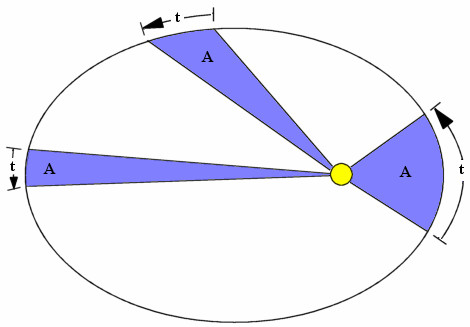
\includegraphics[scale=.3]{imagenes/2leykepler.jpeg}\\
\end{tabular}
\end{frame}
  
  
  
\begin{frame}[fragile]{Un poco de mecánica celeste}
En la dirección radial $\v{u}_r$ la componente de la fuerza es $-\mu/r^2$. Es decir se satisface la ecuación
\[
  \ddot{r}-r\dot{\theta}^2=-\frac{\mu}{r^2}
\]
Notar que esta ecuación entraña dos incognitas $r$ y $\theta$, pero $\dot{\theta}$ puede ser remplazado por $h/r^2$ por la segunda Ley de Kepler.  
Declaremos la variable $h$ que juega un rol importante y reemplacemos $\dot{\theta}$ en la ecuación 
\begin{sageblock}
    h=var('h')
    ed=(a1[0]).subs_expr(theta.diff(t)==h/r^2)
    ed+=mu/r^2   
\end{sageblock}
Resulta
\[\sage{ed}\]

\end{frame}
  
   
\begin{frame}[fragile]{Un poco de mecánica celeste}
Conseguimos una ecuación no lineal de segundo orden para $r$. De los métodos que hemos visto, ninguno se aplica a esta ecuación.  
El truco mágico consiste en considerar la nueva variable dependiente $z=1/r$ y la nueva variable independiente 
$\theta$. 
\begin{sageblock}
  z=function('z',theta)
  r=1/z
  ed2=r.diff(t,2)+mu/r^2-h^2/r^3
\end{sageblock}
Se obtiene
\begin{sagecommandline}
 sage: ed2
-h^2*z(theta(t))^3 + mu*z(theta(t))^2 +
...2*D[0](theta)(t)^2*D[0](z)(theta(t))^2/z(theta(t))^3 -
...D[0](theta)(t)^2*D[0, 0](z)(theta(t))/z(theta(t))^2
...- D[0, 0](theta)(t)*D[0](z)(theta(t))/z(theta(t))^2
\end{sagecommandline}




\end{frame}   


    
\begin{frame}[fragile]{Un poco de mecánica celeste}
En la ecuación resultante, nuevamente aparece $\dot{\theta}$ y además ahora aparece $\ddot{\theta}$. Tenemos que reemplazar
$\dot{\theta}$ por $hz^2$ y $\ddot{\theta}$ por $\tfrac{d}{dt}hz^2$. 

\begin{sageblock}
  theta2diff=(h*z^2).diff(t).\
  subs_expr(theta.diff(t)==h*z^2)
  ed3=ed2.subs_expr\
  (theta.diff(t)==h*z^2,theta.diff(t,2)==theta2diff)
  ed4=(ed3/z^2/h^2).expand()
\end{sageblock}
Resulta
\[\sage{ed4}\]
La ecuación del oscilador armónico. Sabemos resolver esta ecuación y SAGE también!!
\begin{sageblock}
  s=var('s')
  ed5=ed4.subs_expr(theta==s)
  sol1=desolve(ed5,z,ivar=s)
\end{sageblock}
 
\end{frame}    


\begin{frame}[fragile]{Un poco de mecánica celeste}

obtenemos
\[
 \sage{sol1}
\]

Ahora si escribimos $k_1=\rho\cos\omega$ y $k_2=-\rho\sen\omega$ y recordamos que $z=1/r$, deducimos
\[r=\frac{1}{\frac{\mu}{h^2}+\rho\sen(s-\omega)}\]
Llamando $p=\tfrac{h^2}{\mu}$ y $e=\tfrac{\rho h^2}{\mu}$

\boxedeq{r=\frac{p}{1+e\sen(s-\omega)}}{eq:orb_elipse}



\end{frame}    






\begin{frame}[fragile]{Un poco de mecánica celeste}
\textbf{Ejercicio:} La ecuación \eqref{eq:orb_elipse} es la ecuación de una cónica con foco en el origen y excentricidad $e$.
Recordemos que la variable $s$ es el ángulo polar. 

Hagamos algunos gráficos
 
\begin{sageblock}
ListaGra=[]
for e in srange(0,.8,.1):
    ListaGra+=[polar_plot(1/(1+e*cos(s)),\
    (s,0,2*pi),rgbcolor=(e,1-e,0))]
ListaGra+=[polar_plot(1/(1+cos(s)),\
(s,-3*pi/4,3/4*pi),rgbcolor=(e,1-e,0))]
for e in srange(1.2,2,.1):
    ListaGra+=[polar_plot(1/(1+e*cos(s)),\
    (s,-0.65*pi,0.65*pi),rgbcolor=(0,2-e,e-1))]
gra=sum(ListaGra).show()

\end{sageblock}

\end{frame}    

\begin{frame}[fragile]{Un poco de mecánica celeste}

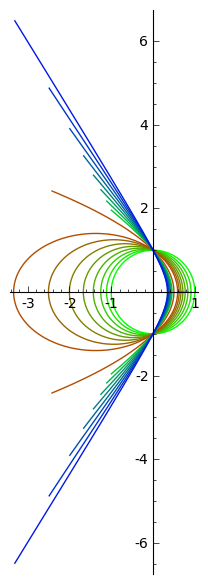
\includegraphics[scale=.5]{imagenes/conicas.png}

\end{frame}  

\begin{frame}[fragile]{Un poco de mecánica celeste}

Hemos logrado encontrar $r$ como función de $\theta$. Esto fue importante, de allí por ejemplo deducimos que las órbitas eran cónicas. No obstante
no hemos logrado resolver aún el problema de los dos cuerpos \eqref{eq:grav},  para ello deberíamos encontrar $\v{r}(t)$, es decir poner a $
\v{r}$ como función de $t$. Esto nos serviría para decir que punto de la órbita ocupa el planeta en unn dado momento.  Este problema no lo desarrollaremos aquí dado 
que su solución se aparte del tema de las ecuaciones diferenciales.
que excede los objetivos de este curso. 



\end{frame}  



\end{document}